\documentclass{beamer}
\usetheme{Madrid}
\usepackage[utf8]{inputenc}
\usepackage[T1]{fontenc}
\usepackage{graphicx}
\usepackage{lmodern}

% Pour enlever le \institute du bas de page
% Rapetisser les noms et date etc dans le footer
\setbeamertemplate{footline}
{
  \leavevmode%
  \hbox{%
  \begin{beamercolorbox}[wd=.333333\paperwidth,ht=2.25ex,dp=1ex,center]{author in head/foot}%
    \
  \end{beamercolorbox}%
  \begin{beamercolorbox}[wd=.333333\paperwidth,ht=2.25ex,dp=1ex,center]{title in head/foot}%
    \usebeamerfont{title in head/foot}\insertshorttitle
  \end{beamercolorbox}%
  \begin{beamercolorbox}[wd=.333333\paperwidth,ht=2.25ex,dp=1ex,right]{date in head/foot}%
    \usebeamerfont{date in head/foot}\insertshortdate{}\hspace*{2em}
    \insertframenumber{} / \inserttotalframenumber\hspace*{2ex} 
   \end{beamercolorbox}}%
  \vskip0pt%
}

\AtBeginSection[]
{
	\begin{frame}
		\tableofcontents[currentsection,hideallsubsections]
	\end{frame}
}

\title{Soutenance Projet Android}
\author{Baptiste Saleil, Julien Pagès, Walid Benghabrit}
\date{\today}

\begin{document}
	\begin{frame}
		\titlepage
		
		\begin{center}
			
\includegraphics[scale=0.25]{logo.png}
		\end{center}
	\end{frame}

	%Plan
	\begin{frame}{Plan}
		\tableofcontents
	\end{frame}

	\section{Introduction}
		% Contexte du projet
		\begin{frame}{Contexte}
			\begin{itemize}
				\item Projet Universitaire
				\item Projet de Master 2
				\item Développement d'une application utilisant des composants d'Android
				\item Découverte des plateformes embarquées
			\end{itemize}
		\end{frame}
		
		% Problématique
		\begin{frame}{Sujet}
			\begin{exampleblock}{Consignes}
				\begin{itemize}
					\item Application de guidage des étudiants au sein du campus 
					\item Utilisation du GPS (localisation, routes)
					\item Placement de marqueurs
					\item Définir et implémenter des fonctionnalités
				\end{itemize}
			\end{exampleblock}
		\end{frame}
		
		\section{Analyse et conception}
		% Choix
		\begin{frame}{Choix}
			\begin{block}{Stratégiques}
				\begin{itemize}
					\item Répartition des tâches
					\item Usage de bibliothèques libres
					\item Utilisation d'un gestionnaire de version
					\item Développement itératif
				\end{itemize}
			\end{block}		
			\pause
			\begin{block}{Conception}
				\begin{itemize}
					\item Exploitation du Hardware (géolocalisation, guidage vocal)
					\item Guidage vers un bâtiment
					\item Liste des différents bâtiments
					\item Recherche textuelle/vocale
					\item Affichage d'objets divers sur la carte (toilettes, machine à cafés...)
					\item Gestion de fichiers de calendrier, guidage automatique
				\end{itemize}
			\end{block}
		\end{frame}
		
		\begin{frame}{Architecture}
			\begin{center}
				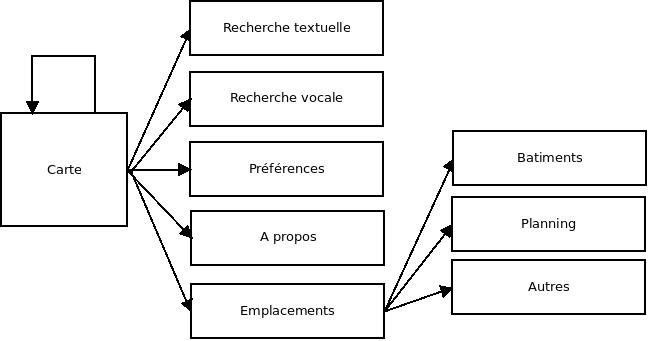
\includegraphics[scale=0.5]{diagram.jpeg}
			\end{center}
		\end{frame}
		
		\begin{frame}
		Persistence des données
			\begin{itemize}
			\item Utilisation de SQLite
			\item Création de nos propres parseurs
			\item Définition de nos propres classes
			\item Sérialisation des classes en BD
			\item Recherche, filtrage, affichage...
			\end{itemize}
		\end{frame}
		
		\begin{frame}
		Découverte de la plateforme
			\begin{itemize}
			\item Définition d'icônes
			\item Changements d'activités
			\item Traduction
			\item Exploitation du hardware
			\end{itemize}
		\end{frame}
	\section{Résultats}
		\begin{frame}
			Vue de base de l'application
			\begin{center}
				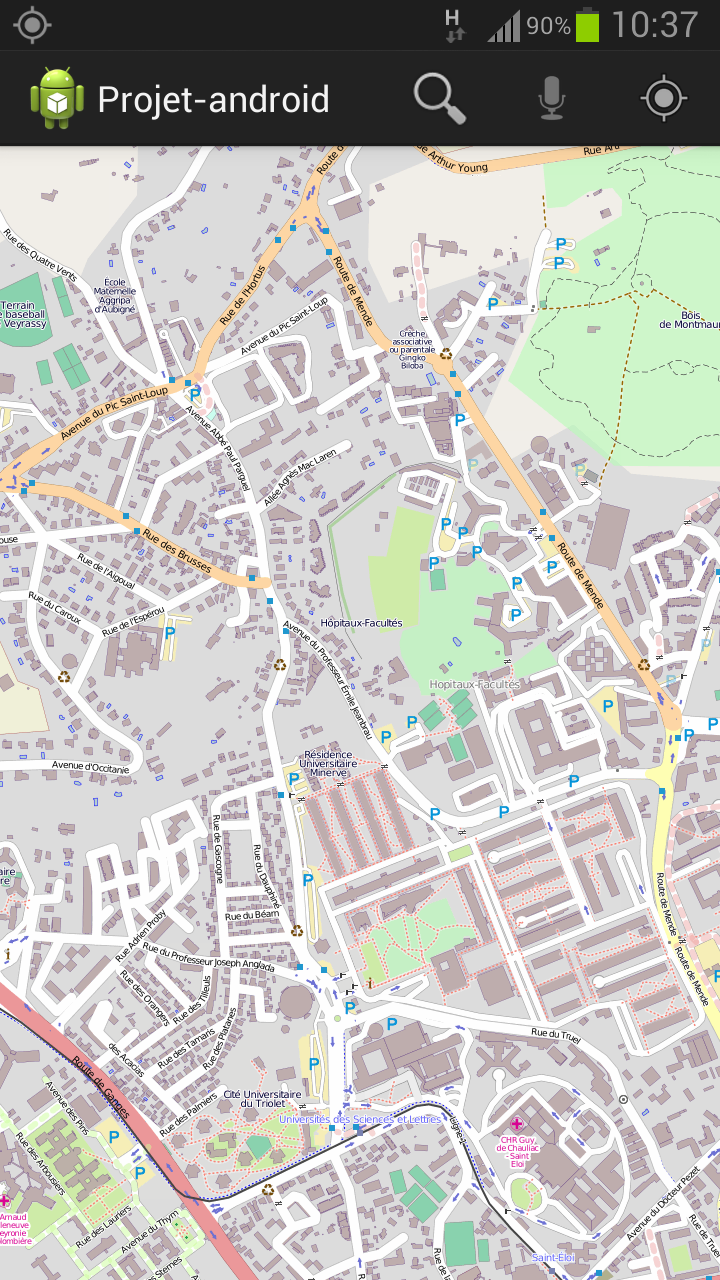
\includegraphics[scale=0.15]{../rapport/carte.png}
			\end{center}
		\end{frame}
		
		\begin{frame}
			Guidage
			\begin{center}
				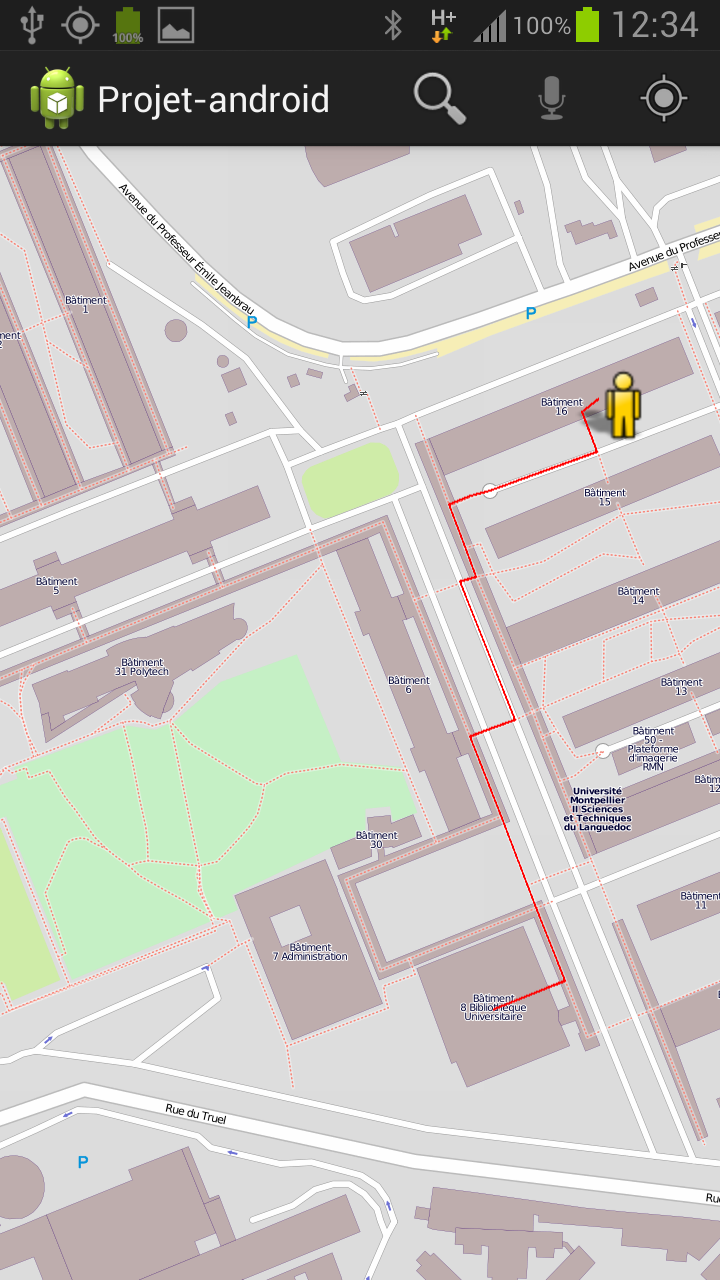
\includegraphics[scale=0.15]{../rapport/guidage.png}
			\end{center}
		\end{frame}
		
		\begin{frame}
			Affichage des marqueurs
			\begin{center}
				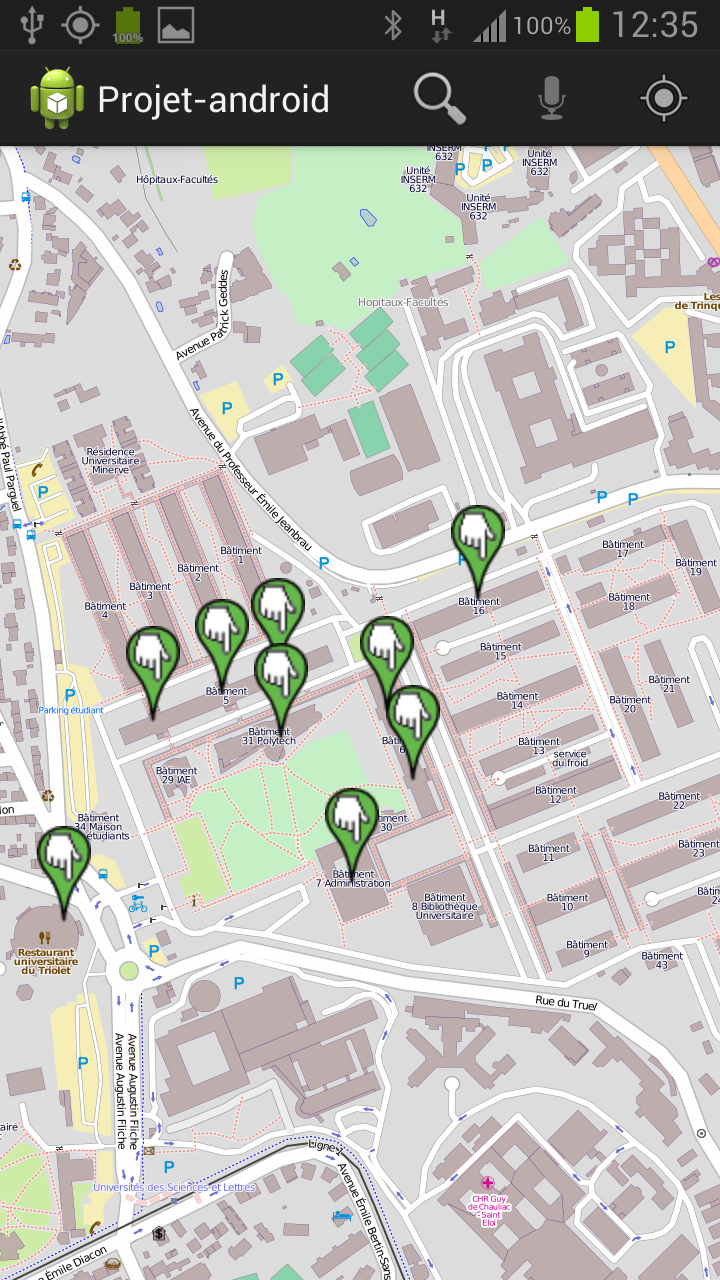
\includegraphics[scale=0.15]{../rapport/marqueurs.png}
			\end{center}
		\end{frame}
		
		\begin{frame}
			Affichage en liste
			\begin{center}
				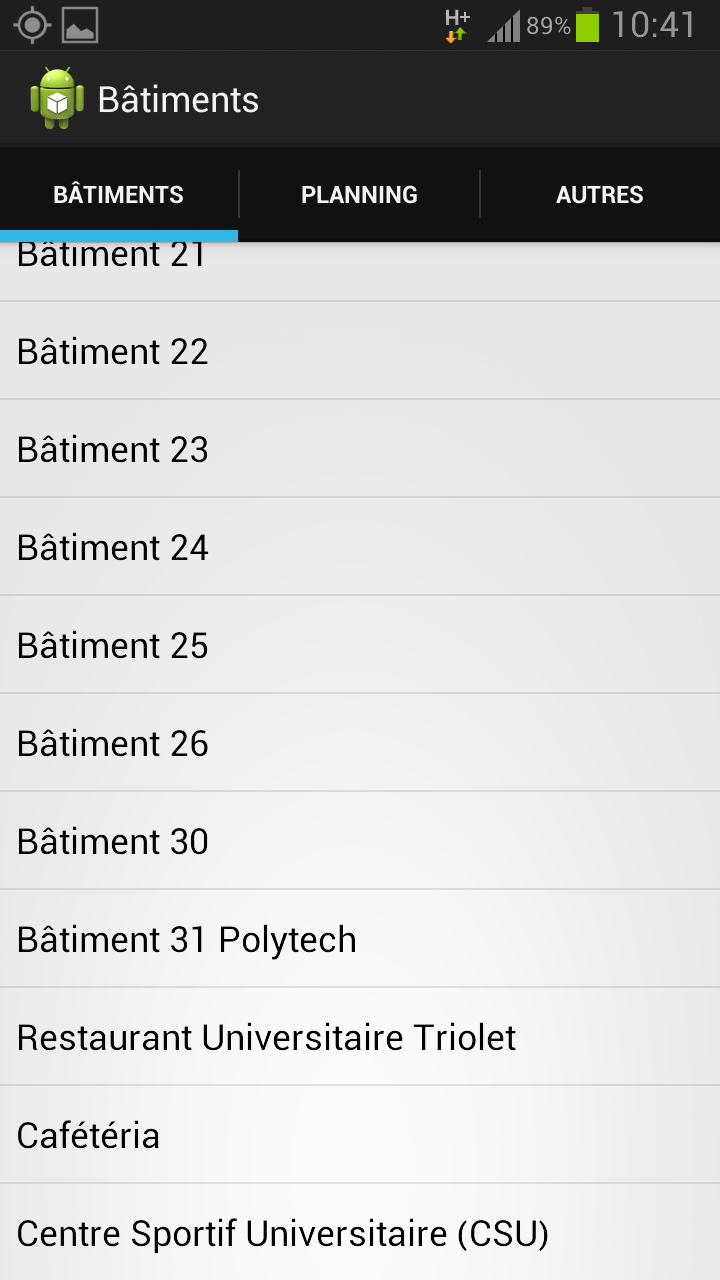
\includegraphics[scale=0.15]{../rapport/liste.png}
			\end{center}
		\end{frame}
	\section{Conclusion}
		\begin{frame}{Difficultés}
			\begin{itemize}
				\item Bibliothèques utilisés peu documentées (OSMdroid)
				\item Multithread
				\item Aspect performances en général
			\end{itemize}
		\end{frame}
		
		\begin{frame}{Bilan}
			\begin{block}{Bilan}
				\begin{itemize}
					\item Cahier des charges respecté
					\item Application fonctionelle, complète
					\item Découverte de nouvelles technologies
					\item Sensibilisation à l'embarqué en général
				\end{itemize}
			\end{block}
			\pause
			\begin{exampleblock}{Ouverture}
				\begin{itemize}
				\item Aller chercher l'emploi du temps directement en ligne
				\item Plus d'éléments répertoriés dans la fac
				\item Amélioration de la recherche en général
				\item Traduction dans plus de langues
				\end{itemize}
			\end{exampleblock}
		\end{frame}
\end{document}
